\chapter{Organización}

\section{Esquema organizativo}

El equipo de trabajo, como se puede ver en la figura ~\ref{fig:org}, se organizará en un comité de
dirección, que será el encargado de valorar el correcto progreso del proyecto, así como de indicar
los posibles cambios necesarios, y un equipo de desarrollo que será el encargado de desarrollar el
proyecto. Además, en la integración del experimento psicológico de Labpsico, el equipo de Labpsico
será parte de la organización del proyecto para validar el progreso.

\begin{figure}[h]
	\centering
	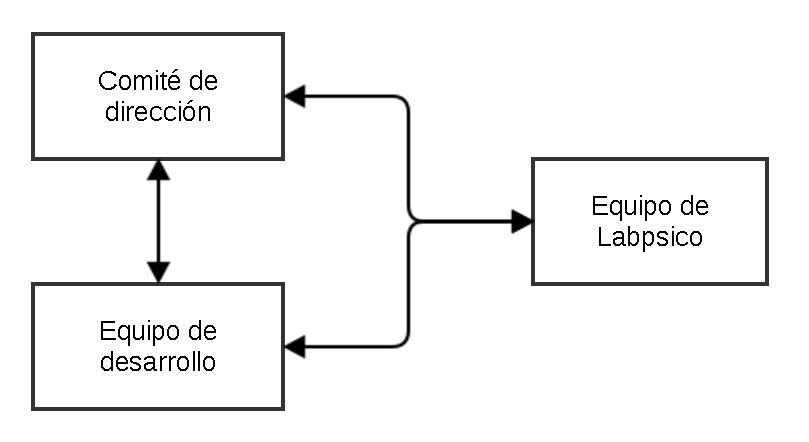
\includegraphics[width=0.7\textwidth]{fig/organizacion}
	\caption{Esquema organizativo del proyecto.}\label{fig:org}
\end{figure}

\section{Plan de recursos humanos}

La jornada laboral será de media jornada, 4 horas y se contará con un recurso que se dividirá en los
siguientes perfiles:

\begin{itemize}
\item Un \textbf{jefe de proyecto}: será el encargado de organizar el proyecto.

\item Un \textbf{programador}: será el encargado del desarrollo de la lógica del producto.

\item Un \textbf{diseñador}: será el encargado de crear una interfaz de usuario intuitiva y simple.

\item Un \textbf{técnico experto en Weblab-Deusto}: será el encargado de la integración con la
plataforma.
\end{itemize}

Se harán reuniones periódicas, cada un máximo de dos semanas para hacer el seguimiento del proyecto.
Para validar los distintos módulos de la aplicación se comprobará si cumple los requisitos
establecidos, y se harán pruebas por miembros voluntarios del equipo de trabajo. La organización del
equipo de trabajo no será jerárquica sino más bien horizontal, para permitir mayor agilidad en el
desarrollo.
